\section*{Βήμα 12}

\noindent Αφού εκπαιδεύσουμε τα μοντέλα μας, τα κάνουμε evaluate με την ακόλουθη συνάρτηση:

\lstinputlisting[language=Python, firstline=273, lastline=289]{../../lab.py}

\noindent Το evaluation γίνεται παίρνοντας τα δεδομένα στο validation set, βάζοντας το καθένα ως είσοδο στο μοντέλο κάθε ψηφίου, λαμβάνοντας από το κάθε μοντέλο τον λογάριθμο τον εκτιμώμενο λογάριθμο της πιθανότητας η είσοδος να αντιστοιχεί σε αυτό το ψηφίο, τυπώνοντας ως έξοδο το ψηφίο που έλαβε την μέγιστη πιθανότητα (λογάριθμο) από το μοντέλο του, και συγκρίνοντας με το πραγματικό ψηφίο αυτής της εισόδου.\\
\\
\noindent Στη συνέχεια, δημιουργούμε διαγράμματα γραμμής και heatmap με το accuracy κάθε διαμόρφωσης μοντέλου στο validation set.

\begin{figure}[H]
	\centering
	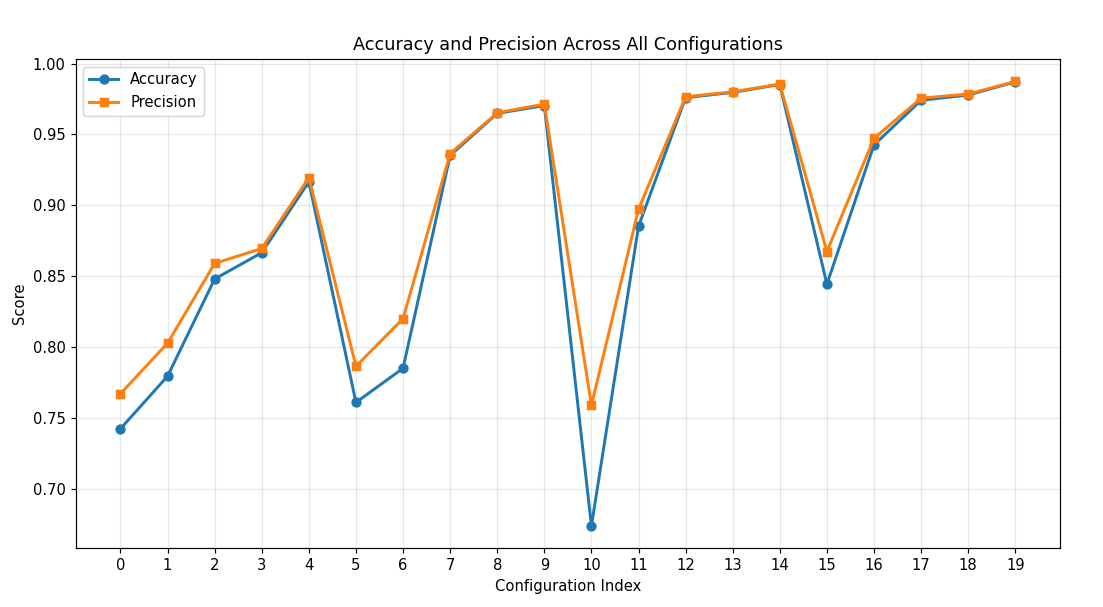
\includegraphics[width=\linewidth]{../../HMM_acc_line_validation.png}
	\caption{Accuracy και Precision κάθε διαμόρφωσης των GMM-HMM μοντέλων.\\
		Φαίνονται 4 φάσεις μήκους 5. Μεταξύ των φάσεων αυξάνεται το n\_states, ενώ εντός κάθε φάσης αυξάνεται το n\_mixtures.}
\end{figure}

\begin{figure}[H]
	\centering
	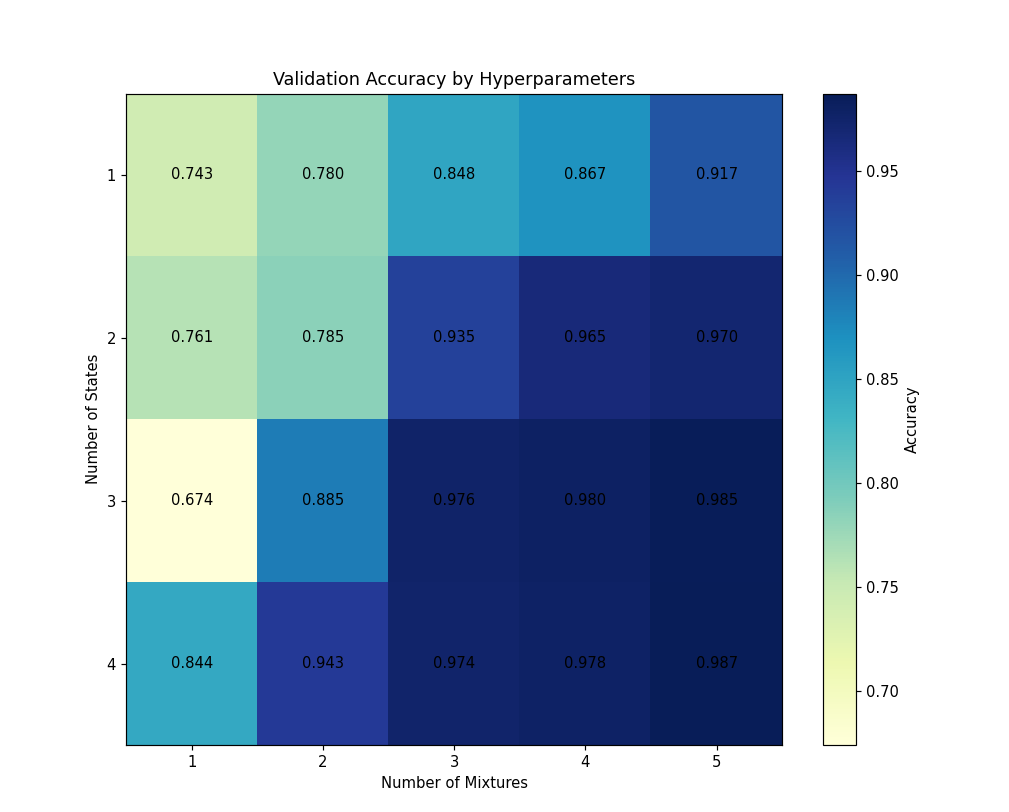
\includegraphics[width=\linewidth]{../../HMM_acc_heat_validation.png}
\end{figure}

\noindent Το καλύτερο μοντέλο είναι εμφανώς αυτό με 4 states και 5 gaussians ανά mixture και επιτυγχάνει accuracy = 98.7\% στο validation set.\\
\\
\noindent Τέλος, υπολογίζουμε την ακρίβεια του καλύτερου μοντέλου και στο testing set (ξανά καλώντας την evaluate αλλά με διαφορετικά δεδομένα). Παρατηρούμε ότι το μοντέλο έχει accuracy = 99\% στο testing set.

\begin{figure}[H]
	\centering
	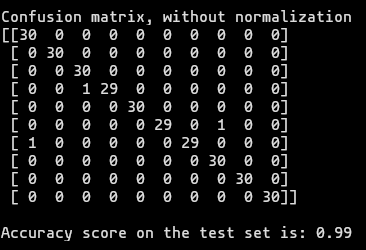
\includegraphics[width=0.5\linewidth]{../../HMM_acc_conf_testing.png}
\end{figure}

\noindent Σημειώνουμε ότι οι δοκιμές που κάνουμε στις παραμέτρους του μοντέλου, εκπαιδεύοντας μόνο στο training set θα έχουν κάποια ακρίβεια στο validation set. Με βάση μόνο αυτήν την ακρίβεια, επιλέγουμε το καλύτερο μοντέλο, και μόνο αφού έχουμε οριστικοποιήσει την επιλογή μοντέλου μας ελέγχουμε την απόδοση στο training set. Από το training set ελαχιστοποιούμε το σφάλμα εκπαίδευσης, από το validation set επιλέγουμε το καλύτερο μοντέλο, και από το testing set υπολογίζουμε εκτίμηση της ακρίβειας του μοντέλου που επιλέξαμε σε δεδομένα που δεν έχει ξαναδεί. Αυτό συμβαίνει, διότι αλλιώς, δηλαδή αν επιλέγαμε το καλύτερο μοντέλο με βάση την ακρίβεια στο training set, τότε ουσιαστικά θα εισάγαμε διαρροή δεδομένων από το testing set στο validation set, και η απόδοσή μας στο testing set δεν θα ήταν αντιπροσωπευτική της απόδοσής μας σε δεδομένα που το μοντέλο μας δεν θα είχε ξαναδεί. Το αντίστοιχο θα συνέβαινε αν χρησιμοποιούσαμε σε οποιοδήποτε σημείο προτού ολοκληρωθεί η εκπαίδευση του κάθε μοντέλο δεδομένα από το validation set. Για αυτόν τον λόγο, προσέξαμε πχ. νωρίτερα στον κώδικα να κάνουμε fit τον Scaler με βάση μόνο τα training data.


